\subsection{Free surface stabilisation}\label{sec:stab}
The benchmark is performed as discussed in \citet{Kaus2010a} and \citet{Thieulot2014}. The domain is square with $L_x=L_y=$ \SI{500}{\km} and a grid resolution
of $200\times200$ elements, each of them containing 16 markers. A buoyant fluid with $\rho_1=$ \SI{3200}{\kg\per\cubic\metre} and $\eta_1=$ \SI{e20}{\pascal\s}
is overlain by a denser fluid with $\rho_2=$ \SI{3300}{\kg\per\cubic\metre} and $\eta_2=$ \SI{e21}{\pascal\s}. The initial interface between the fluids has an
initial sinusoidal shape of 5 km amplitude. Velocity boundary conditions are set to free slip conditions at the sides and no slip at the bottom, while the top
is free surface. The experiment is performed with various fixed time steps, without the use of the Courant number. The vertical position of the free surface at
$x=L_x$ is tracked for each simulation, with or without the stabilisation algorithm.

The results show an instability (drunken sailor effect) increasing the time step in case that the stabilisation algorithm is not activated
($dt=$ \SI{4200}{\year}, green line in Fig. \ref{fig:stab}), as already observed by \citet{Kaus2010a} and \citet{Thieulot2014}. Activating the algorithm the
instability is fixed and the simulation remains stable using time step up to \SI{50000}{\year} (red line in Fig. \ref{fig:stab}). All data can be 
found at \url{https://github.com/aleregorda/Benchmarks/tree/main/Surface_processes/Stabilisation_algorithm}.

\begin{figure}
\centering
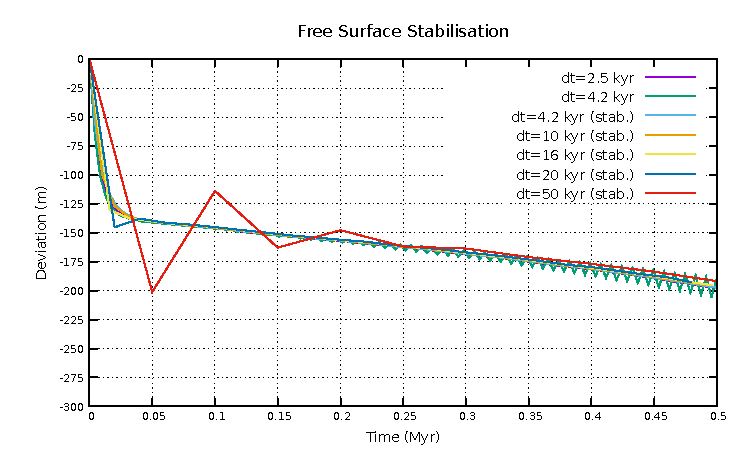
\includegraphics[width=400px]{./Figures/Kaus_random.pdf}
\caption{Evolution of the y coordinate in $x=L_x$ as function of time for different time steps, with and without the stabilisation algorithm.}
\label{fig:stab}
\end{figure}